\chapter{Object Detection from Sliding Windows}
\label{ch:lesson40}

Every classifier so far has focused on images as a whole rather than image patches --- asking ``what \emph{is} this image?,'' assuming it already contains exactly one thing, centered and cropped. Object \textbf{detection} asks a harder question: given an image that contains zero, one, or several objects at unknown locations and scales, find the \emph{location} of each one.

The classic approach is the \textbf{sliding window}: train a classifier for a fixed-size image patch, then slide the classifier across the image to run it at every location (and scale). \citelink{rowleybalujakanade1996}{Rowley, Baluja, and Kanade (1996)} did exactly this with a small neural network as the window classifier. This idea was truly ahead of its time --- one of the first successful uses of a neural net for a real vision task, more than a decade before deep learning's resurgence (Chapter~\ref{ch:lesson37}). This chapter builds the approach end to end: a small window classifier, applied at every position, followed by a key step that any real system needs --- merging duplicate detections.

\section{Step 1: a synthetic ``face'' and a window classifier}

To demonstrate the mechanics, real data isn't needed --- only a class with consistent internal structure (a head outline, two eyes, a mouth, always in the same relative arrangement) versus clutter that lacks that structure (Figure~\ref{fig:l40-1}). Train a small CNN as a pure window classifier: given a fixed-size crop, is there a face filling it, yes or no?

\begin{figure}[h]
\centering
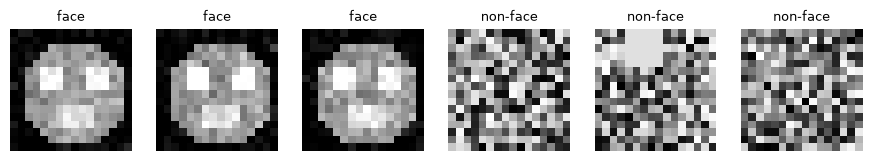
\includegraphics[width=0.85\textwidth]{figures/lesson40_fig01.png}
\caption{Synthetic face examples vs.\ non-face clutter.}
\label{fig:l40-1}
\end{figure}

\begin{lstlisting}
class WindowClassifier(nn.Module):
    def __init__(self):
        super().__init__()
        self.net = nn.Sequential(
            nn.Conv2d(1, 8, 3, padding=1), nn.ReLU(), nn.MaxPool2d(2),
            nn.Conv2d(8, 16, 3, padding=1), nn.ReLU(), nn.AdaptiveMaxPool2d(1),
        )
        self.fc = nn.Linear(16, 1)
\end{lstlisting}

Trained for 300 epochs: window classifier test accuracy $100.0\%$.

\section{Step 2: slide the window across a scene}

Build a larger scene containing two faces at unknown locations plus background clutter (true face centers at $(29.0,19.0)$ and $(48.0,47.0)$), then run the trained window classifier at every position on a dense grid (a \textbf{sliding window}). Each position gets a raw confidence score, which is recorded at that window's center. Since windows can't be centered within \code{win // 2} pixels of the border (a window close to the edge doesn't fit inside the image), the score is not computed within a border strip, shown in gray in Figure~\ref{fig:l40-2}.

\begin{lstlisting}
def sliding_window_scores(model, scene, win=16, stride=1):
    half = win // 2
    scores = np.full(scene.shape, np.nan, dtype=np.float32)
    for y0 in range(0, scene.shape[0] - win + 1, stride):
        for x0 in range(0, scene.shape[1] - win + 1, stride):
            patch = scene[y0:y0+win, x0:x0+win]
            scores[y0 + half, x0 + half] = model(torch.tensor(patch[None, None]).float()).item()
    return scores
\end{lstlisting}

\begin{figure}[h]
\centering
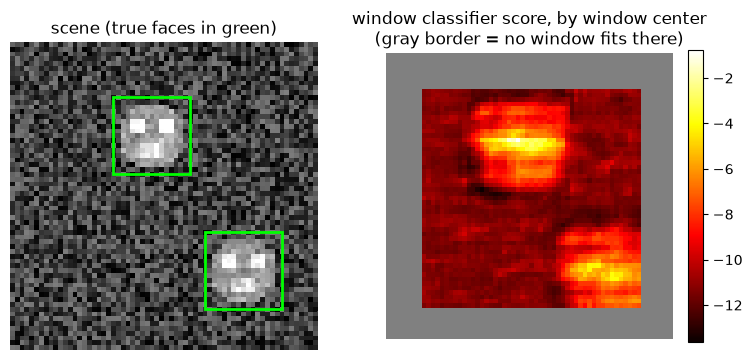
\includegraphics[width=0.9\textwidth]{figures/lesson40_fig02.png}
\caption{The scene (true faces outlined in green) and the window classifier's score map, indexed by window center (gray border = no window fits there).}
\label{fig:l40-2}
\end{figure}

\section{Step 3: threshold, then merge duplicates}

The score map peaks near the true faces, but thresholding produces a \emph{cluster} of detections around each face --- every window that overlaps a face heavily enough scores above threshold. This is precisely the duplicate-detection problem Chapter~\ref{ch:lesson12} first raised for both Canny and the Hough transform: many near-identical hypotheses need to collapse into one. The fix is \textbf{non-maximum suppression (NMS)}: repeatedly keep the highest-scoring remaining detection and discard every other detection that overlaps it by more than an IoU (intersection-over-union) threshold.

\begin{lstlisting}
def nms(detections, iou_thresh=0.3):
    dets = sorted(detections, key=lambda d: -d[4])
    keep = []
    while dets:
        best = dets.pop(0)
        keep.append(best)
        dets = [d for d in dets if iou(best, d) < iou_thresh]
    return keep
\end{lstlisting}

Using a threshold set at the 97.5th percentile of all window scores ($-5.14$): 60 raw detections lie above threshold; NMS collapses these to just 2, landing at $(cx{=}29,cy{=}19)$ and $(cx{=}50,cy{=}49)$ --- one exactly on a true center, the other within a couple of pixels (Figure~\ref{fig:l40-3}).

\begin{figure}[h]
\centering
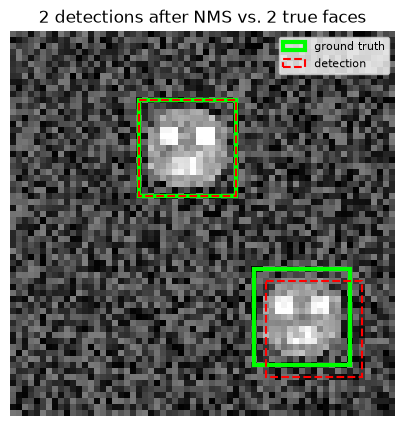
\includegraphics[width=0.5\textwidth]{figures/lesson40_fig03.png}
\caption{2 detections after NMS (red, dashed) vs.\ 2 true faces (green).}
\label{fig:l40-3}
\end{figure}

With this threshold and \code{iou\_thresh=0.3}, NMS collapses the raw detections down to two boxes that closely match the two true face locations. As the exercises below explore, results on other scenes and seeds yield false positives and false negatives, depending on the threshold and other parameter choices.

\section{Handling scale: the image pyramid}

Everything above assumes faces are always exactly $16\times16$, but real faces appear at unknown scales. The solution is Chapter~\ref{ch:lesson11}'s Gaussian pyramid (\code{cv2.pyrDown}): build a stack of the image at multiple resolutions, and run the \emph{same fixed-size} window classifier over every level. A face that's too big for the window at full resolution will fit the window at some coarser pyramid level, since shrinking the image is equivalent to enlarging the effective window size relative to image content.

\section{Viola-Jones}

The Rowley-Baluja-Kanade window classifier (what this chapter just built, in miniature) was computationally heavy at the time. In 1996 (pre-GPUs) evaluating a small neural network at every position and scale of every pyramid level was slow. \citelink{violajones2001}{Viola and Jones (2001)} modified the same sliding-window idea to run in real time by replacing the neural network with a \textbf{cascade} of extremely cheap Haar-like features (the same local sum/difference idea as Chapter~\ref{ch:lesson16}'s Haar wavelet, applied to 2D rectangular regions): a sequence of stages, each a simple threshold on a rectangular-region intensity difference, ordered so that the vast majority of non-face windows get rejected by the \emph{first} stage or two, and only the rare promising windows pay for the full cascade of classifiers. As a result, the cascade's average cost per window is tiny --- which is why Viola-Jones is the algorithm that ended up running live on 2000s-era digital cameras.

OpenCV ships the Viola-Jones cascade as \code{cv2.CascadeClassifier}, pretrained on real faces. Just load an XML file of learned cascade stages and run it. On a real photo of the Apollo 11 crew (Figure~\ref{fig:l40-4}): 4 detections.

\begin{figure}[h]
\centering
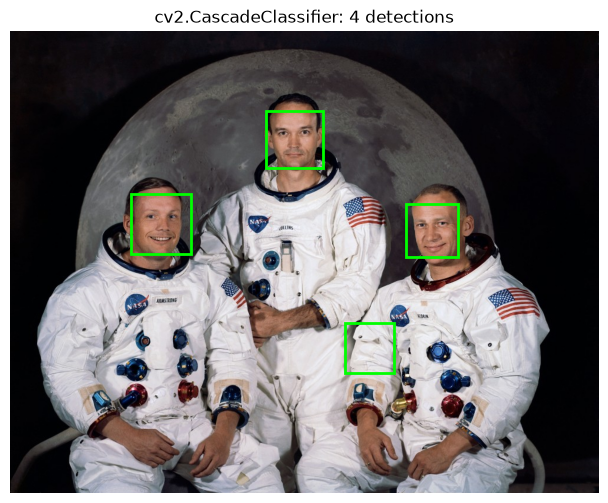
\includegraphics[width=0.75\textwidth]{figures/lesson40_fig04.png}
\caption{\code{cv2.CascadeClassifier} on a real photo: 4 detections. \attrib{Image source: NASA (public domain), via Wikimedia Commons.}}
\label{fig:l40-4}
\end{figure}

All three astronauts' faces (Armstrong, Collins, Aldrin) are found correctly, plus a small false positive on the fabric texture on Aldrin's sleeve. \code{minNeighbors} (how many overlapping detections a region must have) and \code{scaleFactor} (how coarsely the image pyramid steps between scales) trade off false positives against missed faces, playing a role similar to this chapter's NMS threshold.

\subsection*{Exercises}
\begin{enumerate}
  \item Change \code{iou\_thresh} in \code{nms} from $0.3$ to $0.7$. Rerun detection on the scene. Does NMS now under-merge (report more than 2 boxes) or over-merge (miss a face)? Explain why in terms of how much overlap real duplicate detections around the same face actually have.
  \item The threshold here is set from the 97.5th percentile of \emph{this scene's own} score distribution --- a form of cheating, since a real detector doesn't get to see the test scene's scores before deciding. Instead, compute a threshold from the training set's known face/non-face scores only, and check whether it still successfully detects both faces in the scene.
  \item Increase \code{n\_faces} in \code{make\_scene} to 4 and shrink \code{size} to 48 so faces are packed closer together. Does NMS still separate them correctly, or does IoU-based suppression start merging genuinely distinct nearby faces into one detection? At what spacing does it break down?
  \item Lower \code{minNeighbors} on the real Viola-Jones cascade from $5$ to $2$ and rerun. Does the fabric false positive get worse, or do new false positives appear elsewhere? Then try raising \code{minNeighbors} to $8$ --- does it clean up the false positive, and does it cost any true detections?
\end{enumerate}

\vfill
\fullcode{lesson40}{lesson40_object_detection_sliding_windows}
